\section{电流强度}\label{sec:8-1}

\xiaobiaoti{电流强度}
电流不但有方向,而且有强弱。有的电流比较强,有的电流比较弱。
并联在照明电路中的不同的白炽灯泡,发光强弱不同,就是因为通过它们灯丝的电流强弱不同。
怎样来表示电流的强弱呢?我们知道,电荷的定向移动形成电流。
因此,要知道电流的强弱,需要先知道电荷的多少。

电荷是有多有少的。在摩擦起电中,带电体所带电荷越多,它吸引轻小物体的能力就越强。
使带电体接触验电器时,带电体所带电荷越多,验电器的箔片张开的角度就越大。

电荷的多少叫做\textbf{电量}。
电量有个天然的最小单位,这就是电子所带的电量,任何电量都是这个最小单位的整数倍,
但是这个单位实在太小了,为了方便,人们常用一个比它大得多的单位——\textbf{库仑}作电量的单位。
$6.25 \times 10^{18}$ 个电子所带的电量是 1 库仑。

电流通过导体的时候,每秒钟通过导体横截面的电量有多有少,
通过的电量越多,电流就越强,
通过的电量越少,电流就越弱。
电流的强弱是用电流强度来表示的。
\textbf{1 秒钟内通过导体横截面的电量叫做电流强度}。

\begin{enhancedline}
如果用 $I$ 表示电流强度,用 $Q$ 表示通过的电量,$t$ 表示通电时间,那么
$$I = \dfrac{Q}{t} \;\juhao$$
上式中电量 $Q$ 的单位是库仑,时间 $t$ 的单位是秒,电流强度 $I$ 的单位是安培。
如果在 \CJKunderwave{1 秒钟内通过导体横截面的电量是 1 库仑,导体中的电流强度就是 1 安培}。
安培的符号是 A 。
$$ 1 \anpei = \dfrac{1 \kulun}{1 \miao} \;\juhao $$

如果在 10 秒内通过导体横截面的电量是 20 库仑,那么导体中的电流强度
$$ I = \dfrac{Q}{t} = \dfrac{20 \kulun}{10 \miao} = 2\anpei \;\juhao $$
\end{enhancedline}

常用的电流强度单位还有毫安(mA)、微安($\mu$A)。
$$ 1\anpei = 1000 \text{毫安,} $$
$$ 1\text{毫安} = 1000 \text{微安。} $$


\begin{table}[H]
    \centering
    \caption*{一些电流强度值 (安培)}
    \begin{tabular}{w{l}{10em}l}
        电子手表            & $(1.5\text{~}2) \times 10^{-6}$ \\
        晶体管收音机        & $(1\text{~}10) \times 10^{-2}$ \\
        晶体管电视机        & $(1\text{~}3) \times 10^{-1}$ \\
        普通家用白炽电灯    & $\text{约}(1\text{~}3) \times 10^{-1}$ \\
        电子管电视机        & $\text{约} 1$ \\
        汽车上的发电机      & $\text{约} 20$ \\
        大型发电机          & $(0.8\text{~}11) \times 10^3$ \\
        闪电                & $(2\text{~}20) \times 10^4$ \\
    \end{tabular}
\end{table}


\xiaobiaoti{安培表}
测量电路中的电流强度要使用电流表。
刻度盘上以安培为单位的电流表,标着一个字母 A,通常叫安培表(图 \ref{fig:8-1})。

安培表是比较精密的仪器,一定要按照正确的方法去使用,以免损坏。

\begin{figure}[htbp]
    \centering
    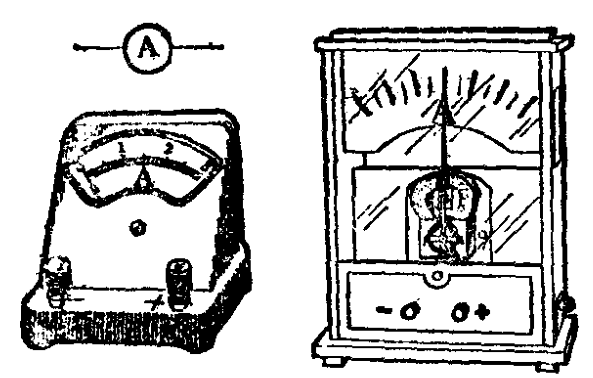
\includegraphics[width=0.5\textwidth]{../pic/czwl2-ch8-1}
    \caption{安培表(左图上方是安培表的符号)}\label{fig:8-1}
\end{figure}

\begin{figure}[htbp]
    \centering
    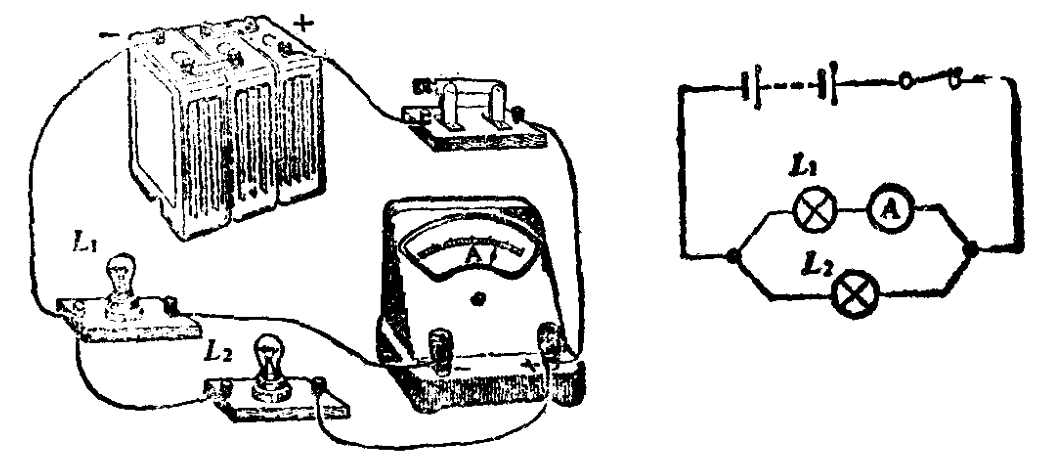
\includegraphics[width=0.7\textwidth]{../pic/czwl2-ch8-2}
    \caption{}\label{fig:8-2}
\end{figure}


如果要测量某部分电路中的电流强度,必须把安培表串联在这部分电路里,让这部分电路的电流全部通过安培表。
例如,在图 \ref{fig:8-2} 中,要测量的是 $L_1$ 支路中的电流强度,所以把安培表串联在 $L_1$ 支路中。

学校里用的安培表,两个接线柱上分别标着 “$+$”、“$-$” 号,
这种安培表的 “0” 点一般在刻度盘的左端(图 \ref{fig:8-1} 的左图)。
将这样的安培表串联到电路里的时候,
\CJKunderwave*{必须使电流从“$+$”接线柱流进安培表,从“$-$”接线柱流出来}。
如果接错了,安培表的指针就要向没有刻度的那边偏转,使安培表损伤。

每个安培表都有一定的测量范围——量程,通过安培表的电流强度如果超出这个范围,安培表会烧坏或损伤。

使用安培表的时候,绝对不允许不经过用电器而将安培表的两个接线柱直接连到电源的两极上,
以免由于电流强度过大而将安培表烧坏。

